\section{História}

\begin{frame}
	\frametitle{Curiosidade}
	\begin{figure}[htpb]
		\centering
		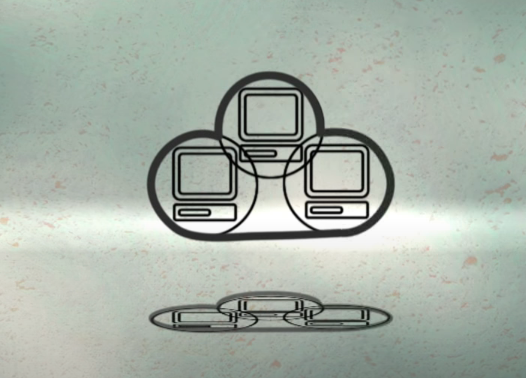
\includegraphics[width=0.6\textwidth]{server_cluster}
		\caption{A cluster of servers drawn in a system diagram \footnote{\href{https://www.youtube.com/watch?v=e3UMvBP2RRo}{Image source link}}}
	\end{figure}
\end{frame}

\subsection{Linha do tempo}

\begin{frame}
	\frametitle{Linha do tempo}
	\begin{center}
		História da computação em nuvem\cite{CCHistory}
	\end{center}
	\hfill
	\begin{scriptsize}
	\begin{bf}
	\begin{center}
		\begin{chronology}[10]{1955}{2010}{12cm}[\textwidth]
			\event[1955]{1965}{1955-1965}
			\event[1970]{1990}{1970-1990}
			\event[1990]{2006}{1990-2006}
			\event{2006}{2006}
			\event[2006]{2010}{2016-2010}
		\end{chronology}
	\end{center}
	\end{bf}
	\hfill
	\begin{itemize}
		\item (1955-1965) Problemas na infraestrutura de TI
		\item (1970-1990) Hypervisors e a internet
		\item (1990-2006) Internet para todos
		\item (2006-2006) Precipitation
		\item (2006-2010) Primeiros dias da computação em nuvem
	\end{itemize}
	\end{scriptsize}
\end{frame}

\begin{frame}
	\frametitle{Linha do tempo}
	\begin{center}
		Problemas na infraestrutura de TI \\ (1955-1965)
	\end{center}
	\hfill
	\begin{scriptsize}
	\begin{bf}
	\begin{center}
		\begin{chronology}[10]{1955}{2010}{12cm}[\textwidth]
			\color{lightgreen}
				\event[1955]{1965}{1955-1965}
		\end{chronology}
	\end{center}
	\end{bf}
	\end{scriptsize}
\end{frame}

\begin{frame}[allowframebreaks]
	\frametitle{Problemas na infraestrutura de TI}
	\begin{itemize}
		\item 1942 - John Vincent Atanasoff construiu o computador ABC
		\item 1960 - Muito caro para aderir os computadores
			\begin{itemize}
				\item Sala inteira para o servidor (Manter temperatura ideal, espaço, etc\dots)
				\item Computador
				\item Funcionários especializados
				\item Problemas para adaptar o software
			\end{itemize}
		\framebreak
		\item Empresas com poder aquisitivo conseguiram aderir os computadores
		\item 1961 - John MacCharty fez uma palestra no MIT
			\begin{itemize}
				\item Computação poderia ser vendida como água ou eletricidade \cite{SimsonTCI}
				\item Mas seria necessário de uma grande evolução tecnológica
			\end{itemize}
	\end{itemize}
\end{frame}

\begin{frame}
	\frametitle{Linha do tempo}
	\begin{center}
		Hypervisors e a internet \\
		(1970-1990)
	\end{center}
	\hfill
	\begin{scriptsize}
	\begin{bf}
	\begin{center}
		\begin{chronology}[10]{1955}{2010}{12cm}[\textwidth]
			\color{lightgreen}
				\event[1970]{1990}{1970-1990}
		\end{chronology}
	\end{center}
	\end{bf}
	\end{scriptsize}
\end{frame}

\begin{frame}[allowframebreaks]
	\frametitle{Hypervisors e a internet}
	\begin{itemize}
		\item Diminiur os custos da adoção do computador
			\begin{itemize}
				\item Múltiplos usuários podem compartilhar o mesmo armazenamento e o poder de processamento da CPU
			\end{itemize}
		\item 1970 - Nasceu a tecnologia da virtualização
			\begin{itemize}
				\item Um host pode ser particionado em VMs
				\item Cada parte pode rodar um código independente
			\end{itemize}
		\framebreak
		\item 1983 - A internet nasceu
			\begin{itemize}
				\item Projeto ARPANet: comunicação de professores de universidades
			\end{itemize}
		\item Arquitetura cliente-servidor conectados por cabos (Internet)
		\item O número de servers cresceram junto com as páginas web
			\begin{itemize}
				\item Os servers se moveram para datacenters
			\end{itemize}
	\end{itemize}
\end{frame}

\begin{frame}
	\frametitle{Linha do tempo}
	\begin{center}
		Internet para todos \\
		(1990-2006)
	\end{center}
	\hfill
	\begin{scriptsize}
	\begin{bf}
	\begin{center}
		\begin{chronology}[10]{1955}{2010}{12cm}[\textwidth]
			\color{lightgreen}
				\event[1990]{2006}{1990-2006}
		\end{chronology}
	\end{center}
	\end{bf}
	\end{scriptsize}
\end{frame}

\begin{frame}
	\frametitle{Internet para todos}
	\begin{itemize}
		\item Empresas precisavam de datacenters maiores
		\item Problemas:
			\begin{itemize}
				\item Ociosidade dos servers (off-season)
				\item Escalabilidade manual e precisava de dispositivos físicos
					\begin{itemize}
						\item Difícil acompanhar o crescimento da aplicação
					\end{itemize}
				\item Atualização e manutenção manuais
				\item Grande distância dos servidores (UX ruim)
			\end{itemize}
	\end{itemize}
\end{frame}

\begin{frame}
	\frametitle{Linha do tempo}
	\begin{center}
		Precipitation \\
		(2006)
	\end{center}
	\hfill
	\begin{scriptsize}
	\begin{bf}
	\begin{center}
		\begin{chronology}[10]{1955}{2010}{12cm}[\textwidth]
			\color{lightgreen}
				\event{2006}{2006}
		\end{chronology}
	\end{center}
	\end{bf}
	\end{scriptsize}
\end{frame}

\begin{frame}[allowframebreaks]
	\frametitle{Precipitação}
	\begin{itemize}
		\item Grandes players (\it{Google, Amazon, eBay, etc\dots})
			\begin{itemize}
				\item Próprio \it{data center}
				\item Centenas/milhares de servers de alta qualidade no mundo inteiro
				\item Começar a alugar essas máquinas
			\end{itemize}
		\item 2006 - "Cloud Computing" introduzino como forma de aluguel de poder computacional
		\item AWS - primeira provedora de cloud
		\item Sonho de John McCharty foi realizado depois de 50 anos
	\end{itemize}
\end{frame}

\begin{frame}
	\frametitle{Linha do tempo}
	\begin{center}
		Primeiros dias da computação em nuvem \\
		(2006-2010)
	\end{center}
	\hfill
	\begin{scriptsize}
	\begin{bf}
	\begin{center}
		\begin{chronology}[10]{1955}{2010}{12cm}[\textwidth]
			\color{lightgreen}
				\event[2006]{2010}{2016-2010}
		\end{chronology}
	\end{center}
	\end{bf}
	\end{scriptsize}
\end{frame}

\begin{frame}[allowframebreaks]
	\frametitle{Primeiros dias da computação em nuvem}
	\begin{itemize}
		\item Por 6 anos a AWS estabeleceu seu monopólio na área de nuvem
		\item Computação em nuvem $\rightarrow$ empresa focam no desenvolvimento
			\begin{itemize}
				\item Os dados são criptografados e seguros
				\item Dados são armazenados com redundância em nuvem
				\item Escalabilidade
				\item De fácil deploy
				\item Alta disponibilidade
			\end{itemize}
	\end{itemize}
\end{frame}
